\section{Arbeitsgrundlagen}

\subsection{Messung der Lichtgeschwindigkeit nach Michelson}

In diesem Versuch wird die  Lichtgeschwindigkeit  nach der Methode von Michelson
(Abbildung  \ref{fig:michelson})  gemessen. Dabei  wird  ein  Laserstrahl  durch
verschiedene  Linsen,  Spiegeln  und Blenden  hin-  und  zur\"uckgeschickt.  Ein
Spiegel,  $DS$, wird mit einem Motor  bei  verschiedenen,  bekannten  Drehzahlen
rotiert. Da das Licht endlich  schnell  ist,  wird der Drehspiegel einen anderen
Winkel haben nach Zur\"uckreflektieren des Lichtstrahls  vom Endspiegel $ES$ und
verursacht somit  eine  Verschiebung des Zur\"uckkommenden Laserstrahls. Ist die
Distanz  zwischen Endspiegel und Drehspiegel $D_2  +  S_2$  sowie  die  Drehzahl
$\omega$   bekannt,   so   kann   durch    Messung    der    Verschiebung    die
Lichtgeschwindigkeit berechnet werden.

\begin{figure}[H]
    \center
    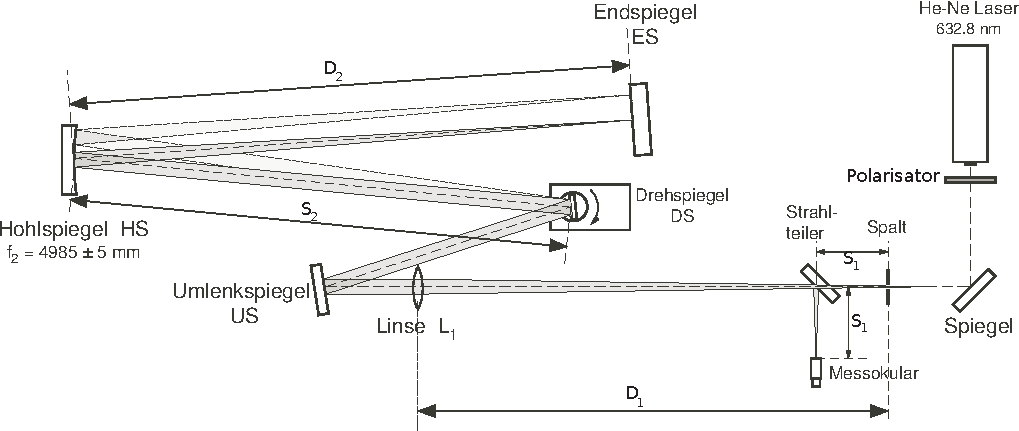
\includegraphics[width=\textwidth]{images/michelson.pdf}
    \caption{Versuchsaufbau nach Michelson. Auszug aus der Aufgabenstellung.}
    \label{fig:michelson}
\end{figure}

Der  Versuch  nach  Michelson kann mit einer \"Aquivalenten  Linsenkonfiguration
dargestellt werden, wie in der Abbildung \ref{fig:linsenkonfig} ersichtlich ist.

\begin{figure}[H]
    \center
    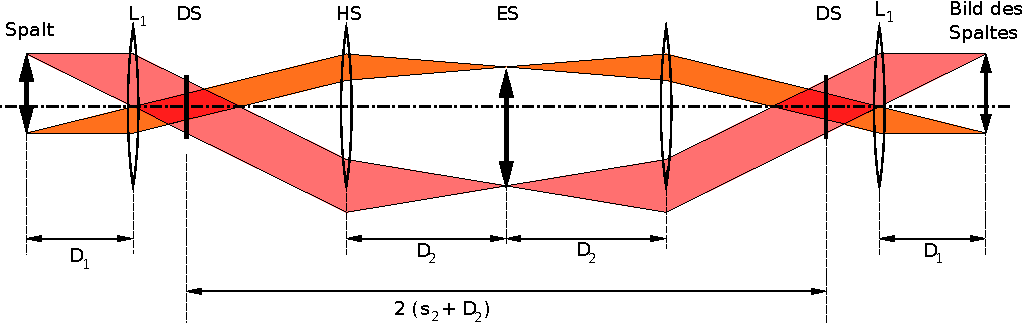
\includegraphics[width=\textwidth]{images/linsenkonfig.pdf}
    \caption{\"Aquivalente Linsenkonfiguration des Versuchs. Auszug aus der Aufgabenstellung}
    \label{fig:linsenkonfig}
\end{figure}

Bei rotierendem Spiegel findet  das  vom  Endspiegel  zur\"uckkehrende Licht den
Drehspiegel wegen der  endlichen  Laufzeit  um  einen  kleinen  Winkel  $\delta$
gedreht

\begin{equation}
    \delta = \omega \cdot \Delta t = \omega \cdot \frac{2(S_2 + D_2)}{c}
    \label{eq:delta}
\end{equation}

wobei  $\omega$  die Kreisfrequenz des Drehspiegels und $\Delta t$ die  Laufzeit
des  Lichtes  vom  Drehspiegel zum Endspiegel  und  zur\"uck  bezeichnen.  Diese
Drehung des Spiegels  hat  eine  Richtungs\"anderung  der  B\"undelachse  um den
Winkel   $2\delta$  (Reflexionsgesetz,   Abbildung   \ref{fig:reflexionsgesetz},
$\alpha=\alpha'  \to  2\delta$)  und  damit eine seitliche Verschiebung $x$  des
Bildes des Spaltes zur Folge.

\begin{figure}[H]
    \center
    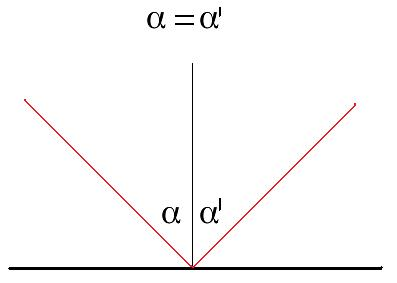
\includegraphics[width=.4\textwidth]{images/reflexionsgesetz.jpg}
    \caption{Reflexionsgesetz}
    \label{fig:reflexionsgesetz}
\end{figure}

F\"ur   das   Verst\"andnis    des    Strahlenganges    ben\"otigen    wir   die
Abbildungsgleichung und  den  Abbildungsmassstab  $\beta$  f\"ur d\"unne Linsen.

\begin{equation}
    \frac{1}{f} = \frac{1}{g} + \frac{1}{b}
    \hspace{15mm}\textrm{und}\hspace{15mm}
    \beta = \frac{B}{G} = \frac{b}{g}
    \label{eq:optik}
\end{equation}

Wobei $f$ die Brennweite, $g$ die Gegenstandsweite (Abstand Linse - Gegenstand),
$b$  die  Bildweite,  $B$  die  Bildgr\"osse  und  $G$  die  Gegenstandsgr\"osse
bezeichnen.

Da die Kleinwinkeln\"aherung $\sin\theta \approx \tan\theta \approx \theta$ in
unserem Falle sicher zul\"assig ist, gilt
\begin{equation}
    2\delta = \frac{x}{D_1}
    \label{eq:kleinwinkelapprox}
\end{equation}
und damit
\begin{equation}
    c = 4\omega \cdot \frac{(S_2 + D_2)D_1}{x}
    \label{eq:deltaumformung}
\end{equation}

Diese Formel muss f\"ur die linearen Regression umgeformt und mit  einem  Offset
$x_0$  angepasst  werden, weil die Millimeterschrauben einen unbekannten  Offset
hat.
\begin{equation}
    x = \frac{1}{c} \cdot 8\pi f \cdot D_1(S_2 + D_2) + x_0 \hspace{15mm}\textrm{oder}\hspace{15mm} x = b \cdot f + x_{02}
    \label{eq:lichtgeschwindigkeit}
\end{equation}

Wobei $f$ die Drehfrequenz des Motors ist und $b = \frac{1}{c} \cdot 8\pi\cdot D_1(S_2+D_2)$.

Eine   sch\"one   Visualisierung   der   Verschiebung   in   Abh\"angigkeit  des
einstrahlwinkels  kann  in  der   Abbildung  \ref{fig:lense-simulation}  gesehen
werden\footcite{ref:linsen-simulation}. Die  weissen  Linien  strahlen mit einem
anderen Winkel als die gelbe Linien in die Linse und verursachen dementsprechend
eine vertikale Verschiebung des Bildes.

\begin{figure}[H]
    \center
    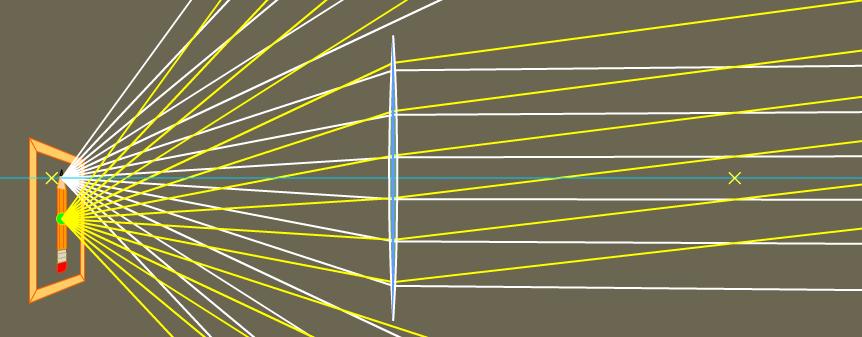
\includegraphics[width=.8\textwidth]{images/lense-simulation.png}
    \caption{Verhalten von Lichtstrahlen bei unterschiedlichen Einstrahlwinkel}
    \label{fig:lense-simulation}
\end{figure}

Der gr\"osste Beitrag zur Unsicherheit der  Lichtgeschwindigkeitsmessung  stammt
von  der Brennweite der Linse $f_1$ respektiv der  Einstellung  von  $D_1$.  Aus
diesem Grunde wird die  Verschiebung des Okulars in Funktion des Winkels, um den
der r\"uckkehrende Laserstrahl verdreht ist, gemessen. Auf einem Arm der L\"ange
$l_{Arm} = (0.50000\pm0.00005)\textrm{m}$ ist ein planer Spiegel  montiert.  Mit
Hilfe einer Mikrometerschraube wird der  Arm  und damit der Spiegel kontrolliert
um   die   entsprechende   Achse   verdreht.   Bei   einer    Verstellung    der
Mikrometerschraube um $z$ resultiert damit ein Winkel
\begin{equation}
    \varphi_{Spiegel} = \arctan{\frac{z}{l}} \approx \frac{z}{l}
\end{equation}

\begin{figure}[H]
    \center
    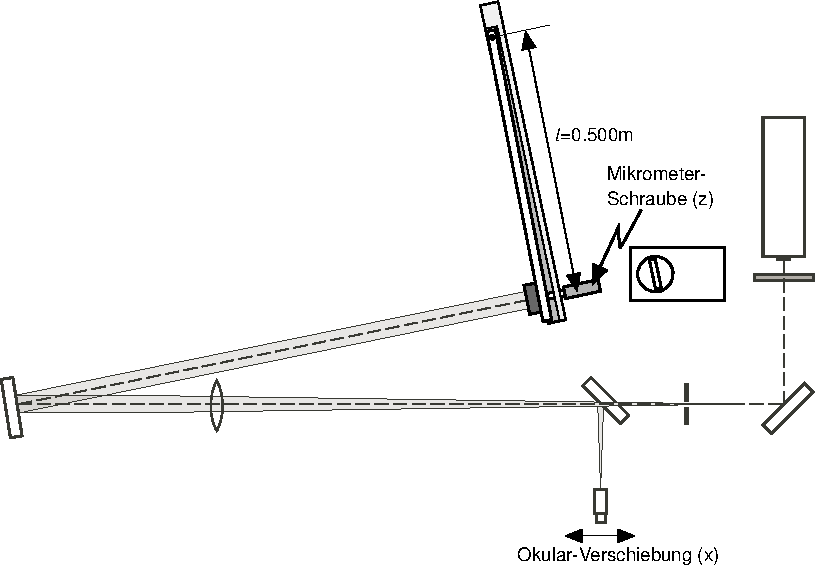
\includegraphics[width=.8\textwidth]{images/kalibration.pdf}
    \caption{Messanordnung Kalibration}
    \label{fig:kalibration}
\end{figure}

Auch hier gilt f\"ur die lineare Regression die Formel
\begin{equation}
    x = a \cdot \varphi_{Spiegel} + x_{01} = \frac{a}{l} + x_{01}
    \label{eq:kalibration-a}
\end{equation}

Setzt man das in der Formel  \ref{eq:lichtgeschwindigkeit} ein, erh\"alt man mit
$\delta = \varphi_{Spiegel}$
\begin{equation}
    \delta = \frac{x - x_{01}}{a} = \frac{b \cdot f + x_{02} - x_{01}}{a} = \frac{b}{a} \cdot f + \frac{x_{02}-x_{01}}{a}
\end{equation}

Gem\"ass Formeln \ref{eq:kleinwinkelapprox} und \ref{eq:deltaumformung} gilt:
\begin{equation}
    \delta = 4\pi f \cdot \frac{S_2 + D_2}{c} + \delta_0
\end{equation}
und folglich
\begin{equation}
    \frac{b}{a} \cdot f = 4\pi f \cdot \frac{S_2 + D_2}{c}
\end{equation}

L\"ost man nach $c$ auf, kriegt man die endg\"ultige Formel:
\begin{equation}
    c = 4\pi\frac{a}{b}(S_2 + D_2)
    \label{eq:lichtgeschwindigkeit_genauer}
\end{equation}

Damit konnte  die  \textbf{gesch\"atzte},  systematische  Unsicherheit von $D_1$
ausgeschlossen werden -- sie wurde ersetzt  durch  die zus\"atzliche statistisch
\textbf{berechnete} Unsicherheit der Steigung $a$.


